Open Computing Language Specification (OpenCL) is an open royalty-free standard for general purpose parallel programming \cite{openclspec} designed to be independent of platform and vendor, whether it be CPU, GPU or other class of accelerator. A detailed investigation of OpenCL and comparison with CUDA can be found in \cite{fagerlund2008}. The OpenCL standard consists of an architecture, an API and a programming language. The architecture is a model of the environment that the computations are performed in, including computational devices such as GPUs and a host system such as a x86 platform that contains the devices. The API is an interface for the host system to build, launch and coordinate parallel computations on the devices. The programming language is a version of the C programming language intended for writing the programs, termed \emph{kernels}, that are executed in parallel on the devices.

A readily available implementation of OpenCL is provided by Nvidia based on their CUDA architecture \cite{cudaprogguide}. There are over one hundred million GPUs sold that can execute CUDA programs. Additionally, AMD also has support for OpenCL as part of their ATI Stream technology \cite{streamreleasenotes}. So there is lots of hardware out there to exploit.

\subsection{OpenCL Architecture}

	The OpenCL architecture defines models for the host system and its computation devices, how the parallel computations are enqueued and executed, and the memory hierarchy on the devices.

	\subsubsection{Platform Model}
	
		Figure \ref{fig:opencl_platform} depicts the OpenCL platform model. The \emph{host} system is connected to one or more \emph{devices}. The devices consist of one or more \emph{compute units} that have a number of \emph{processing elements}. These processing elements do the actual computations. An example of a host system is a x86 desktop computer. Typical devices include GPUs, digital signal processors (DSPs), IBM and Sony's CELL BE processors and even multicore CPUs.
	
		\begin{figure}[h]
		\centering
		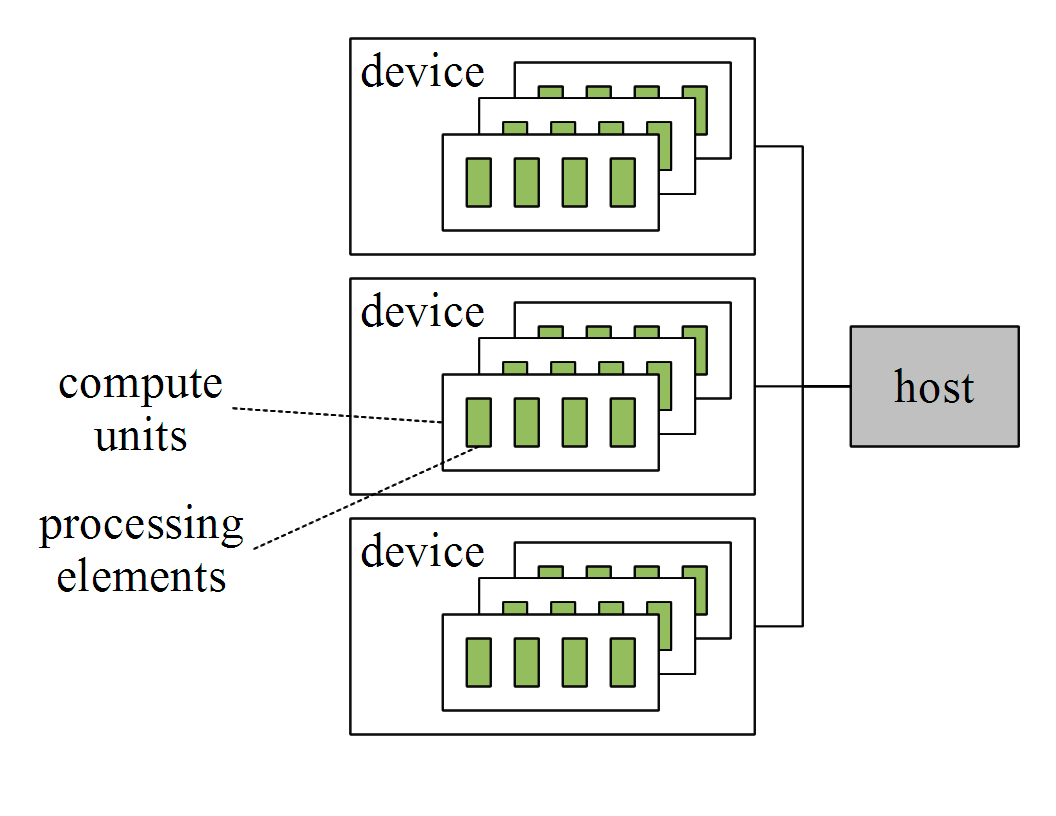
\includegraphics[height=0.35\textheight]{graphics/platform_model.png}
		\caption{OpenCL platform model}
		\label{fig:opencl_platform}
		\end{figure}
	
	\subsubsection{Execution Model}
		
		Figure \ref{fig:opencl_execution} shows the OpenCL execution model. The model is based on the single-instruction multiple-data model where the same operations are performed on different pieces of data. In OpenCL terminology, a \emph{work-item} is a thread that executes a \emph{kernel}. The kernel is written in the OpenCL C-based programming language, which will be described later. Work-items are organized in one, two or three dimensional \emph{work-groups}, and all the work-groups make up a \emph{NDRange} which is an index space in the same number of dimensions as the work-groups. Each work-item has a unique index in this \textit{NDRange}.
		
		\begin{figure}[h]
		\centering
		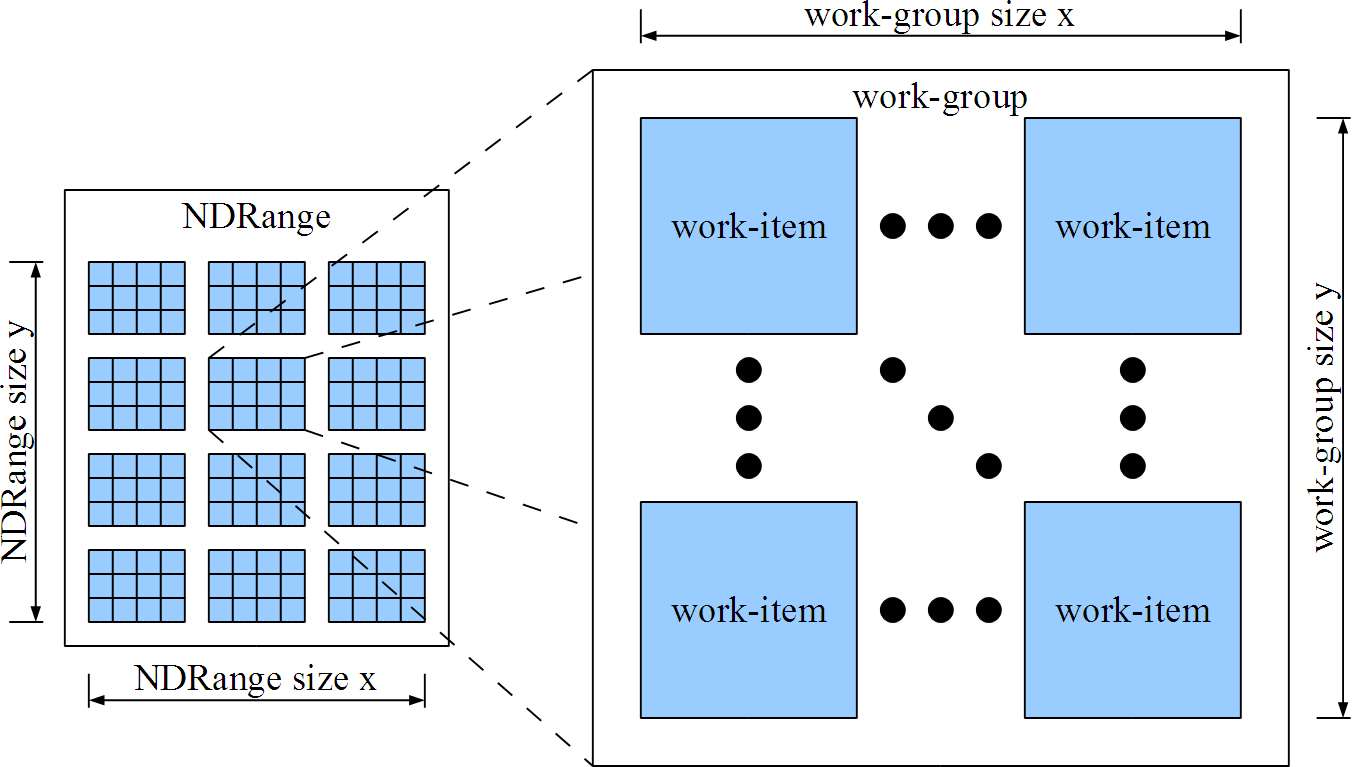
\includegraphics[width=1\textwidth]{graphics/execution_model.png}
		\caption{OpenCL execution model}
		\label{fig:opencl_execution}
		\end{figure}
		
		The execution of parallel kernels, memory transfers and synchronization in OpenCL is organized through \emph{command queues}. The tasks are called \emph{commands}, and are inserted into queues to be performed on or in association with a device. The order of execution can be either synchronous (\emph{in-order}) or asynchronous (\emph{out-of-order}). When in-order, the commands are launched and completed in the order they appear in the queue. When out-of-order, the commands are launched in order, but are not guaranteed to complete in order. The execution environment is defined by a \emph{context} which holds all the objects used during execution, such as devices, memory and command queues. Figure \ref{fig:command_queues} shows a context containing command queues that are mapped to devices.
		
		\begin{figure}[h]
		\centering
		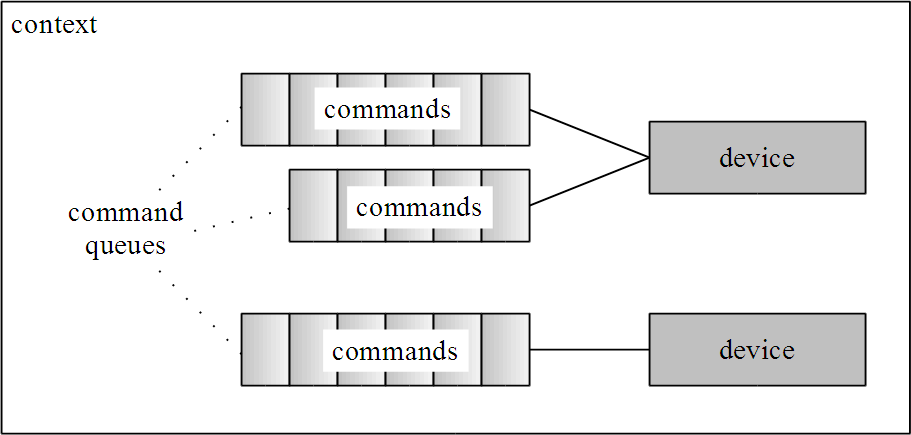
\includegraphics[height=0.25\textheight]{graphics/command_queues.png}
		\caption{OpenCL command queues and devices}
		\label{fig:command_queues}
		\end{figure}
	
	\subsubsection{Memory Model}
	
		Figure \ref{fig:opencl_memory} shows the OpenCL memory model. The model is closely tied to the platform model. The main memory on the device is the \emph{global memory}, which together with the read-only \emph{constant memory} is read- and writeable by the host system. Global and constant memory may be cached on the device. Each compute unit has a \emph{local memory} with the scope of individual work-groups, and each processing element has a \emph{private memory} where data with local scope to individual work-items is stored. Private and local memory are not directly accessible from host.
	
		\begin{figure}[h]
		\centering
		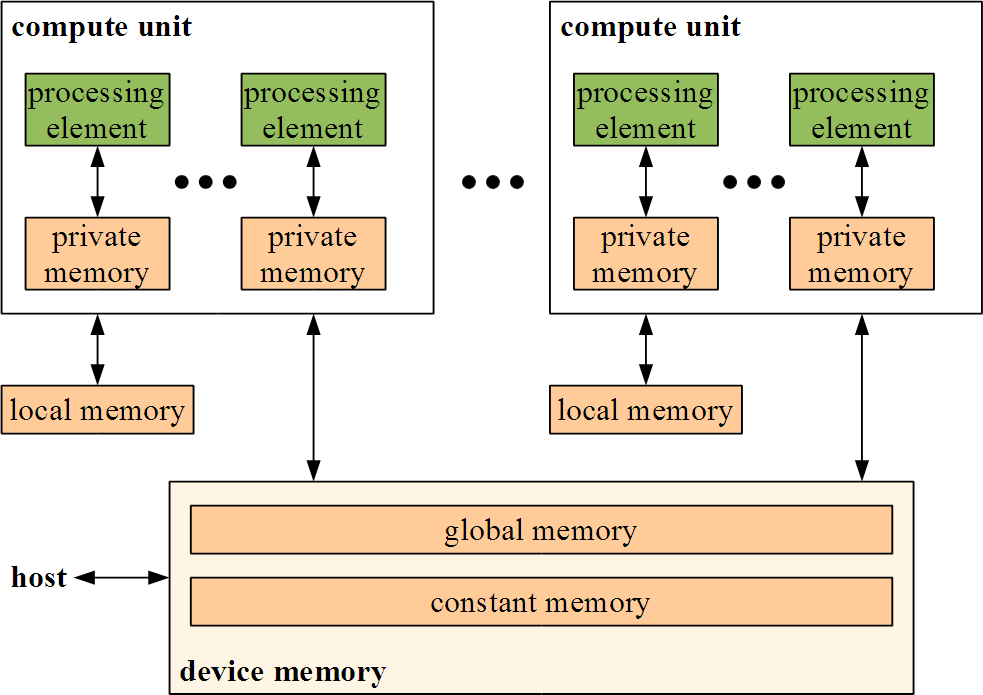
\includegraphics[width=0.9\textwidth]{graphics/memory_model.png}
		\caption{OpenCL memory model}
		\label{fig:opencl_memory}
		\end{figure}
		
\subsection{OpenCL \textit{vs.}\ CUDA}

	Historically, Nvidia's CUDA precedes OpenCL. CUDA was initially launched as a host API and programming model for Nvidia's GPUs. It's popularity made it a \emph{de facto} standard for GPGPU development. Nvidia has taken this a step further and introduced a GPU architecture dubbed the CUDA architecture, and Nvidia's OpenCL implementation runs on the CUDA architecture. Even though CUDA is an architecture, the CUDA API and programming model still exists and is heavily used, and the OpenCL architecture clearly resembles the CUDA architecture. Thus, at the time of writing, OpenCL is an alternative to the CUDA API and programming model. However, Nvidia has implemented the OpenCL standard on top of their CUDA architecture, and in a similar fashion AMD has implemented OpenCL on their ATI Stream technology.
	
	Some major concepts in OpenCL are analogue to concepts in CUDA. For readers experienced with CUDA, Table \ref{table:opencl_vs_cuda} shows CUDA terminology and corresponding equivalent in OpenCL.
	
	\begin{table}[h]
	\centering
	\small
	\begin{tabular}{| l l |}
		\hline
		\textbf{OpenCL terminology} & \textbf{CUDA terminology} \\
		\hline
		\hline
		kernel & kernel \\
		host & host \\
		NDRange & grid \\
		work-item & thread \\
		work-group & block \\
		global memory & global memory \\
		constant memory & constant memory \\
		local memory & shared memory \\
		private memory & local memory \\
		compute unit & stream multiprocessor \\
		processing element & core \\
		image & texture \\
		\hline
	\end{tabular}
	\caption{OpenCL \textit{vs.}\ CUDA terminology}
	\label{table:opencl_vs_cuda}
	\end{table}

\subsection{Host Programming in OpenCL}

	OpenCL provides a host API for building, launching and coordinating parallel computations on devices. It is also possible to extract platform dependent parameters such as memory sizes, maximum work-item sizes and other platform capabilities. This section explains how to use memory, program and kernel objects from the host system, and how to perform synchronization of the parallel computations. For a complete overview, see \cite{openclspec}.

	\subsubsection{Using Memory Objects}
	
		A \emph{memory object} is a part of device memory together with its attributes. By creating memory objects, the host allocates memory on the device. There are two types of memory objects. \emph{Buffers} are sequential arrays of scalar data types such as integers or floating point numbers, and are accessed as a series of bytes. \emph{Images} are two- or three- dimensional arrays for the purpose of containing images such as textures. An important difference between images and buffers is that images are accessed through \emph{samplers} with defined mechanisms for out-of-range coordinates, interpolation between values and filtering. This section will focus on buffer objects.
		
		Creating a buffer object is performed by the \texttt{clCreateBuffer} function:
		
		\begin{verbatim}
		cl_mem clCreateBuffer(cl_context context,
		                      cl_mem_flags flags,
		                      size_t size,
		                      void * host_ptr,
		                      cl_int * errorcode_ret)
		\end{verbatim}
		
		where \texttt{context} is the OpenCL context that will contain the buffer; \texttt{flags} are one or more flags defining attributes of the buffer as given in Table \ref{table:buffer_flags}; \texttt{size} is the buffer size in bytes and \texttt{host\_ptr} is an optional host memory pointer that is used depending on the flags given. The function returns a device memory pointer to the allocated buffer. \texttt{clCreateBuffer} also returns an error code in \texttt{errorcode\_ret} that is not equal to 0 if something went wrong, as most of the other OpenCL API calls also do.
		
		\begin{table}[h]
		\centering
		\begin{tabular}{| p{0.3\textwidth} p{0.65\textwidth} |}
			\hline
			\multicolumn{1}{|c}{\textbf{Flag}} & \multicolumn{1}{c|}{\textbf{Description}} \\
			\hline
			\hline
			\texttt{CL\_MEM\_READ\_WRITE} & Default flag. Buffer is read and written by kernels \\
			\texttt{CL\_MEM\_WRITE\_ONLY} & Write-only access from kernels \\
			\texttt{CL\_MEM\_READ\_ONLY} & Read-only access from kernels \\
			\texttt{CL\_MEM\_USE\_HOST\_PTR} & Use previously allocated \texttt{host\_ptr} as the storage area for the buffer instead of device memory \\
			\texttt{CL\_MEM\_ALLOC\_HOST\_PTR} & Allocate \emph{new} memory on host instead of device \\
			\texttt{CL\_MEM\_COPY\_HOST\_PTR} & Copy data from given \texttt{host\_ptr} to new buffer \\
			\hline
		\end{tabular}
		\caption{OpenCL buffer flags}
		\label{table:buffer_flags}
		\end{table}
		
		\clearpage
		
		Reading and writing buffer objects is performed by the \texttt{clEnqueue[Read|Write]Buffer} functions:
		
		\begin{verbatim}
		cl_int clEnqueue[Read|Write]Buffer(cl_command_queue cmd_queue,
		                                   cl_mem buffer,
		                                   cl_bool blocking,
		                                   size_t offset,
		                                   size_t size,
		                                   void * ptr,
		                                   cl_uint num_events,
		                                   cl_event * event_list,
		                                   cl_event * event)
		\end{verbatim}
		
		where \texttt{cmd\_queue} is the command queue that enqueues the read/write operation, \texttt{buffer} is the buffer object of \texttt{size} bytes and \texttt{blocking} is true/false depending on if the function should be blocking or not. If blocking is enabled, the function will not return until reading/writing has completed. \texttt{offset} is an offset into the buffer object to write or read from and \texttt{ptr} is a pointer to the location on the host to be written to or read from by the procedure.
		
		All functions that enqueue commands optionally have an associated \emph{event object} returned via the parameter \texttt{event}, that can be used to query for the status of the command or wait for its completion (if non-blocking). Furthermore, \texttt{event\_list} can contain a list of \texttt{num\_events} events that needs to be completed before this command is executed.
		
	\subsubsection{Using Program and Kernel Objects}
	
		An OpenCL \emph{program} is a set of kernels that can be built (compiled and linked) and be executed on specified devices. The kernel is usually defined by a string of code in the OpenCL C-based programming language, but can also be a previously compiled binary. The approach described here takes kernels as code strings. The program is created with the \texttt{clCreateProgramWithSource} function and built with the \texttt{clBuildProgram} function, respectively. For clarity, their argument lists are not stated explicitly here, but can be found in \cite{openclspec}.
		
		When the program is built, it is possible to create, set arguments to, and execute \emph{kernel objects} with the functions \texttt{clCreateKernel}, \texttt{clSetKernelArg} and \texttt{clEnqueueNDRangeKernel}. To create a kernel, a successfully built program and a kernel name is supplied. The total size of the arguments cannot exceed a platform dependent maximum (e.g.\ 4352 bytes for Quadro FX5800). Kernels are enqueued on a command queue like the buffer read/write operations. When enqueueing a kernel, the size and dimensionality of the \textit{NDRange} that it will operate on must be specified. A \emph{global work size} is given in $n$ work dimensions and defines the total number of work-items in the \textit{NDRange}. An $n$-dimensional \emph{local work size} is also given such that the size in each dimension evenly divides the corresponding sizes in the global work size. The local work size defines the work-group size. Events can be used for the kernel commands just like with buffer operations mentioned above.
	
	\subsubsection{Host Synchronization}
	
		The previously mentioned event system handles fine-grained synchronization between specific commands in the command queue. Each command can optionally have an associated event, and other commands may depend sequentially on zero or more events before execution can take place.
		
		For global synchronization in a command queue, the host can use the \texttt{clFLush} and \texttt{clFinish} functions. The former requires all commands in a queue be issued to their associated device, but does not have to guarantee that they complete before the function returns. The latter also blocks until they have completed, resulting in a full synchronization of commands.

\subsection{Device Programming in OpenCL}

	A kernel that executes in parallel on a device is written in the OpenCL C-based programming language. This language is based on the C99 standard, but with specific extensions and restrictions. For details, we refer to \cite{openclspec}. The same kernel will be executed in parallel by potentially thousands of work-items in a \textit{NDRange}. An example of a $N \times N$ matrix multiplication kernel can be found in Figure \ref{fig:opencl_kernel}. The kernel is written so that each work-item computes one value of the output matrix product, implying a two-dimensional \textit{NDRange} of size $(N, N)$.
	
		\begin{figure}[h]
		\centering
		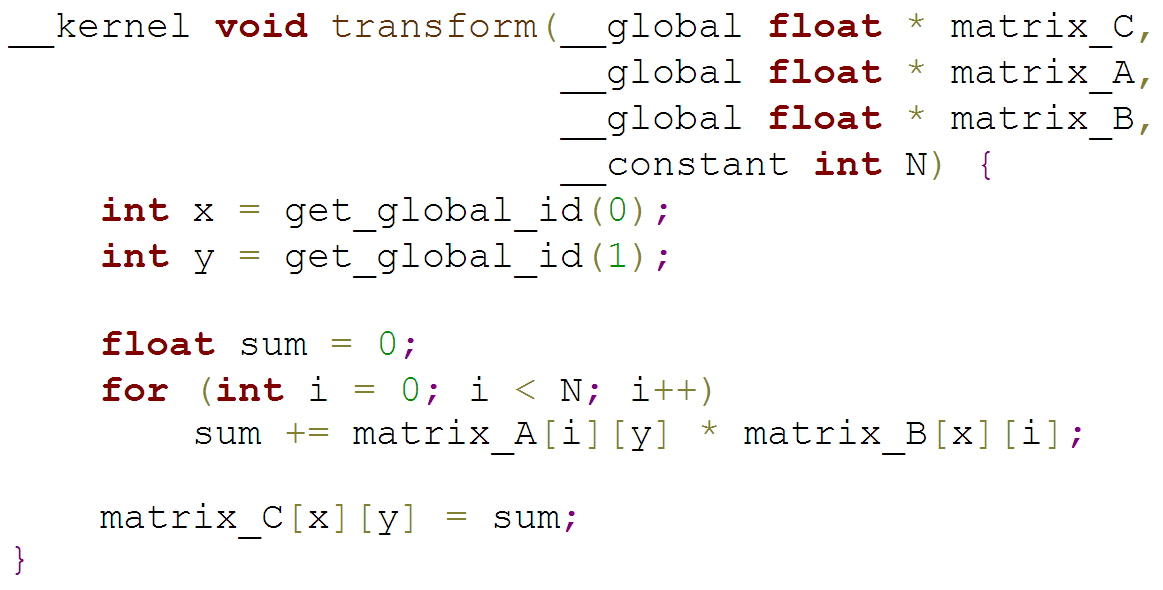
\includegraphics[height=0.27\textheight]{graphics/opencl_kernel.png}
		\caption{OpenCL matrix multiplication kernel}
		\label{fig:opencl_kernel}
		\end{figure}
	
	The OpenCL C-based programming language supports vector arithmetic with integer or floating point vectors of 2, 4, 8 and 16 elements. A number of built-in functions are provided for scalar and vector math, queries about \textit{NDRange} dimensions and work-item index, and for local or global synchronization. Some restrictions for use of the C99 standard apply, and these include: no recursion, use of \texttt{stdio} routines or external variables.